% Copyright (c) 2014,2016,2018 Casper Ti. Vector
% Public domain.

\chapter{相关文献}
% vim:ts=4:sw=4
本章对本研究的相关工作进行回顾与讨论,首先是该可视化所依赖的大型显示设备上的相关感知研究,其次是前人在多分辨率技术框架下曾做出的的不同尝试,最后是对该可视化的基础形式词云的综合介绍。

\section{大型显示设备}
\subsection{大屏可视化}
一些工作通过实验证证实了基于大型显示设备(以下简称``大屏'')的可视化的有效性,为我们在大屏上设计多分辨率词云的动机提供了一定的依据。首先,人们能够适应在大屏上高信息密度的数据可视化。Yost和North~\supercite{Yost2006}的定量研究表明,尽管大型高分辨率显示设备展示的信息更多,但用户在大屏完成基础可视分析任务的耗时与小型设备相比没有显著差异。其次,当需要呈现的信息量较多时,用户也相对青睐于视觉信息密度高单一的大屏设置,而不是小屏限制下的的多层渐进可视分析架构~\supercite{Lam2007}。Andrews等人~\supercite{Andrews2010}观察到,大屏所能展示的更多信息为用户检索数据提供了一定的线索,让他们快速获取更多细节,能有效降低他们的记忆负担。最后,大屏也创造了更为丰富的交互空间,包括手势以与物理移动~\supercite{Badam2016} 。大屏自然地提供了一个``聚焦+细节''(Focus + Context)的界面,有利于对数据的探索:用户从远处可看到可视化的整体概览,而稍加移动靠近屏幕时即可观察到特定的细节。这对某些可视分析任务具有独特的优势。例如,当用户需要搜索定位特定区域时,在大屏前的移动会显著快于在常规笔记本显示屏上的鼠标缩放平移~\supercite{Ball2005}。 

\subsection{人对大屏的感知}

我们简要回顾过往相关的实验与研究,以理解在设计大屏双分辨率词云时所需要考虑的因素。
\begin{figure}[htbp]
	\centering
	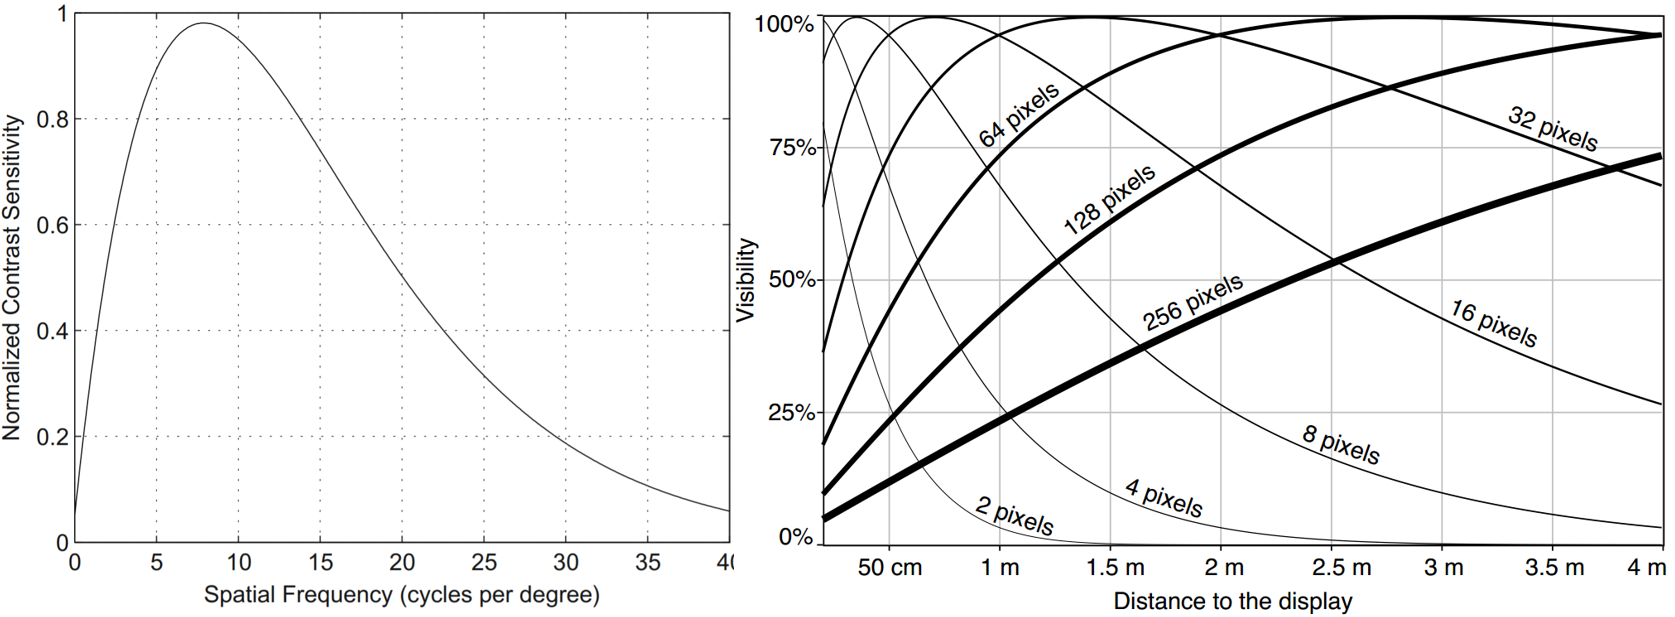
\includegraphics[width=\textwidth]{figures/function.png}
	\caption{左:一个典型的CRF模型~\supercite{Bull2014},横轴为正弦波的空间频域,纵轴为视觉敏感性指标。右:大屏可视范围,横轴为人与显示设备距离,纵轴为可见最小像素~\supercite{Isenberg2013}。}
	\label{fig:function}
\end{figure}

大屏上内容的可分辨性受多种要素影响,如人的视力、视敏度等。一般而言,高对比度的物品会比低对比度的物品更易于分辨。对比-敏感方程~\supercite{Bull2014}(Contrast-Sensibility Function,简称 CRF,见图~\ref{fig:function})拟合了人对不同频率的正弦光栅图的识别阈值的实验结果,反映了视觉神经元对图片对比度的敏感性,表明人的视敏度在3$\sim$4  cpd\footnote{cpd,即cycles per degree,描述视界中正弦光栅图出现的次数,衡量图像特征的空间频率。}时达到峰值,到60 cpd后完全不可见。Isenberg等人~\supercite{Isenberg2013}在大型显示设备~\footnote{该大屏由8×4个30寸显示设备构成,各为2560×1600像素,100ppi。}上用类似的光栅图测试了距离与可见度的关系(见图~\ref{fig:function}),发现不同的特征具有不同的最佳距离,对2或4 ppc的小型特征,它们的可见性在稍近处达到峰值后迅速下降。相反地,对128或256 ppc的大型特征,它们在近处不可见,而到两米外的稍远处维持稳定可见。而对于8$\sim$64 ppc的中等特征,它们具有不同的峰值点与理想可视区域~\footnote{ppc,即pixels per cycle,描述正弦光栅图中一个周期所占像素值。$cpd = \pi / (360tan^{-1}(\frac{p}{2d}ppc))$。}。进一步与普通显示器的对比表明,大屏具有独特的稳定可视距离,而对于一般的显示器而言,只有在60cm处对2$\sim$4 ppc的特征才能达到峰值。这一特性为我们希望人们在不同距离下观察到不同可视化的初始想法提供了可能。

此外,人在大屏上的视觉感知具有一定的局限性。尽管人的视野跨越了170°,但只有以视锥顶点为中心向外张开的20°至40°才是人理想的阅览视角~\supercite{Swaminathan1997}。对于大屏,人们同样倾向于关注40°以内的视野范围,当显示的内容过宽,他们往往会调整自己与屏幕的距离以避免重复的头部移动以及可能的视角扭曲~\supercite{Isenberg2012}。


\section{多分辨率技术}
视觉的产生是因为光线传入视网膜后刺发感光细胞,激发大脑皮层对特定空间频域的并行化处理,由此识别出对应特征。大量心理学研究表明,人的视觉系统对信息的处理具有不同的尺度~\supercite{Joubert2007}。而这种尺度的选择会依人们所需要执行的任务要求发生改变。Olivia和Schyns通过实验发现,在分类任务下,视觉系统会关注于信息量最高的尺度~\supercite{Oliva1997}。本研究所谓的“多分辨率”指的是基于观察者距离界面的不同距离、视角,在同一个静态视图中以不同的分辨率编码信息。以下我们梳理并分析目前我们所知的散见于各学科领域基于多分辨率框架下的工作,探讨他们对多分辨率词云研究的借鉴意义与局限。


\subsection{多分辨率可视化}
多分辨技术能够让观众通过物理位置的变换来动态改变观察视图,因而能够自然地支持信息可视化中奉行的``先概览,通过聚焦和过滤进行筛选,最后提供细节信息''的交互准则~\supercite{Shneiderman96}。然而,目前较少工作利用到了这一技术,主要有频域滤波和图形嵌套方法,该方向尚有很大的研究空间。

\paragraph{频域滤波}Olivia和Schyns~\supercite{Olivia2006}基于他们进行视觉系统信息处理尺度研究实验时所使用的多分辨率技术,在后来综合提出了混合图像的图形学方法,开创了基于频域滤波的多分辨率技术。即通过空间频域滤波,保留远处可见图片A的低频通道,以及近处可见的图片B的高频通道,再利用透明度通道将A与B叠加~\supercite{Baudisch2004},得到同时显示不同细节程度的图片。尽管他们为混合图像构想了四种应用类型,包括揭示同一空间随时间的变迁、动态人像表情、精细纹理混合和文字加密,但他们主要关注于单一或具并列关系的图像,没有考虑编码多层次的信息。特别地,尽管他们从加密的角度特别探讨了文字的多分辨率问题,用随机添加低频噪音的方式防止旁人从远处偷窥文本,但这与我们试图在双重距离范围内使文本清晰可辨大相径庭。此前Majij等人~\supercite{Majaj2002}也在研究字符识别与文字属性(如字体、字号、噪音)的关系时,创造出了同时具有四重分辨率的单字符混合图(见图~\ref{fig:nres}),一定程度上说明了多分辨率方法对字符同样有效。不过,他们着眼于单个字符,而人们对词云的感知是整体性的,还涉及到多文本的共同作用,本研究将更为细致地去考察人们对多分辨率词云的认知感受。

受到混合图像的启发,Isenberg等人\supercite{Isenberg2013}提出了混合图像可视化的概念,指出在大屏上展示静态的混合可视化有助于多人合作可视分析场景。他们在细致分析墙面规模树图、点线图、双刻度散点图与折线图的案例后,进一步探讨了大屏数据可视化中的多分辨率设计准则与任务支持(见图~\ref{fig:nres}),一定程度上说明了多分辨率可视化的广阔应用前景。正是这一工作启发了我们在大屏上同时展示双分辨率下的词云,本研究将在渐进式展现文本数据这一任务的驱动下填补多分辨率词云设计的空白。


\begin{figure}[htbp]
	\centering
	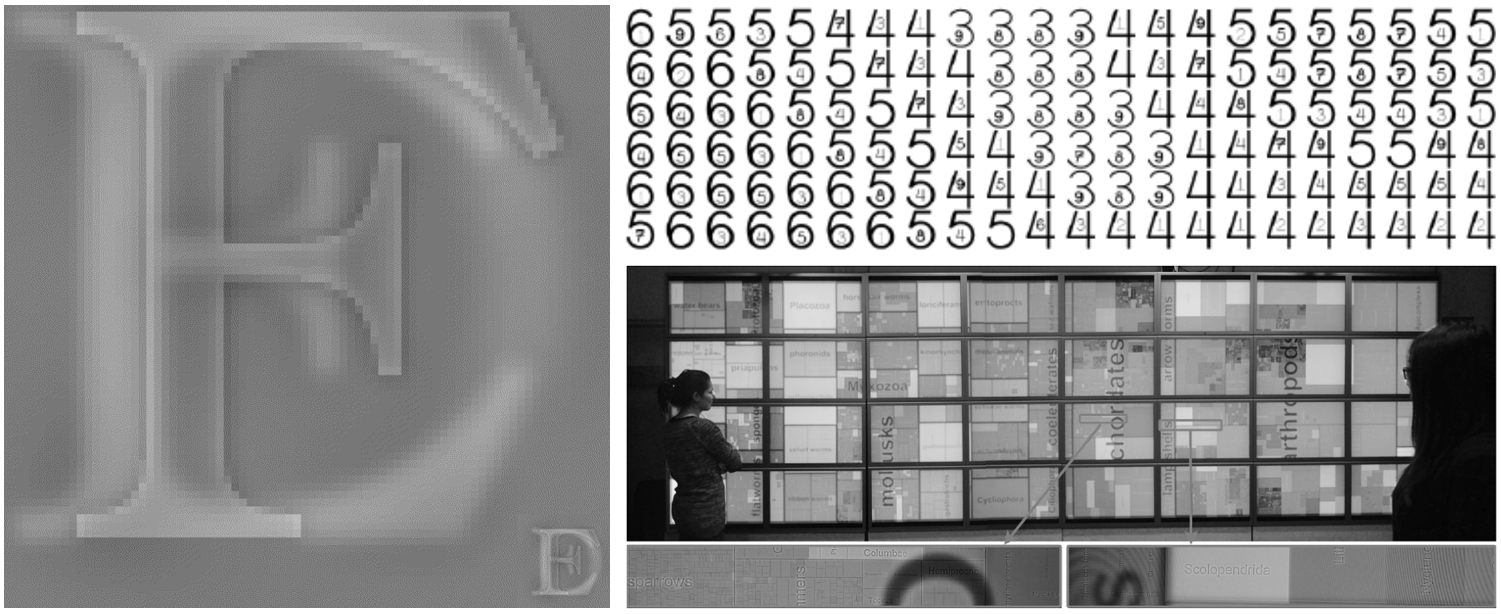
\includegraphics[width=\textwidth]{figures/nres.png}
	\caption{依距离变化可视层级的多分辨率可视化。左:具有四重分辨率的字符设计,由近及远分别是C、D、E、F~\supercite{Majaj2002};右上:FatFont设计示例~\supercite{Miguel2012};右下:大屏上的多分辨率树图~\supercite{Isenberg2013}。}
	\label{fig:nres}
\end{figure}


\paragraph{嵌套图形}另一个类似于本研究思路的可视化案例还有FatFont~\supercite{Miguel2012}(见图~\ref{fig:nres}),这是一种在半色调(Half-toning)~\supercite{Ostromoukhov1995}的基础上利用特殊字体设计来可视化数值的方法。它通过嵌套的方式将高位数字置于最外层,并用字体粗细编码数值大小,使得从远处看时,特定区域的墨点密度能够反映此处的对应信息,构成点画(Stipling)~\supercite{Gortler2019};从近处看时,准确的数值指标能够直接获取。它对罗马数字进行了再设计,适用于空间型数据的可视化,是对视觉通道~\supercite{Munzner2014}的延伸;而本研究侧重于探索常规排列的字符集,以不同的分辨率编码词云,使其相互作用来辅助文本分析。



\subsection{图形排样}
计算机图形学中的非真实感渲染~\supercite{ThomasStrothotte2002}旨在以计算的方式重现艺术化的表现形式。图形排样属于这一领域的子方向,主要研究以特定图案或纹理样式作为最小单元而构成具有审美性的图形。按照最小单元类型,这种方法可进一步分为基于图案碎片的图像拼接(Mosaicking)与基于字符文本的图像诗(calligram)。

\paragraph{图像拼接}参考Battiato等人的综述~\supercite{Battiato2007},图像拼接的方法主要有两种途径:(1)先分解原始图像,再重建产生特殊碎片效果,如马赛克墙饰;(2)从较大的碎片集合中选取元素拼凑为待拟合的图像。其中,最接近本文的多分辨率词云概念的是后者,特别是一种基于不规则图形的拼图式图像拼接,因为字符是不规则的。一大类算法是采用的是优化的观点。以Jigsaw Image Mosaicking~\supercite{Kim2002}算法为代表,它定义了一个由空隙、颜色、重叠、图样变形综合作用的能量函数,通过最小化基础图形排布引发的开销得到解决方案。类似地,Dalal等人~\supercite{dalal2006}通过最小化距离度量与空隙面积来均衡化基于Voronoi区域的分割。而另一大类方式则是基于搜索。如Blasi等人~\supercite{Gallo2006}先对图片进行分割,再在备选图集中匹配最优碎片并进行图像处理使其接近于背景图像。

\paragraph{文字诗}在涉及文字的自动化排布问题中,总体而言研究的数目比较少,其最终效果也和人为创作的文字诗略有区别。我们归纳出了目前存在的三种方向(见图~\ref{fig:calligram})。

\begin{enumerate}
	\renewcommand{\labelenumi}{(\theenumi)}
	\item 通过扭曲字符来适应形状限制。Zou等人~\supercite{Zou2016}根据指定的形状轮廓计算出文字布局的路径,并在沿路径排列字符后通过特定的指标优化矢量字符控制点的位置,使字符尽可能填充区域并保持可识别。不过,这一方法需要基于大量训练数据来得到衡量变形字符可识别性的损失函数并据此优化,因而难以运用于在中文等字符库巨大的语言。类似的工作还有\parencite{Xu2007,Chi2018}等。
	\item 字符艺术。Xu等人\supercite{Xu2010}以\texttt{Ascii}字符做为图形的``像素'',通过纵横排布,使之尽可能接近原始图像的线描。
	\item 基于区域向量场排布。Moharik等人~\supercite{Moharik2011}计算了外层图形轮廓所张成的向量场,由此生成语料文段排列的路径集合,以此排列大段文字,并通过轻微调整每一行的高度使其更多地填充图形。
\end{enumerate}


\begin{figure}[htbp]
	\centering
	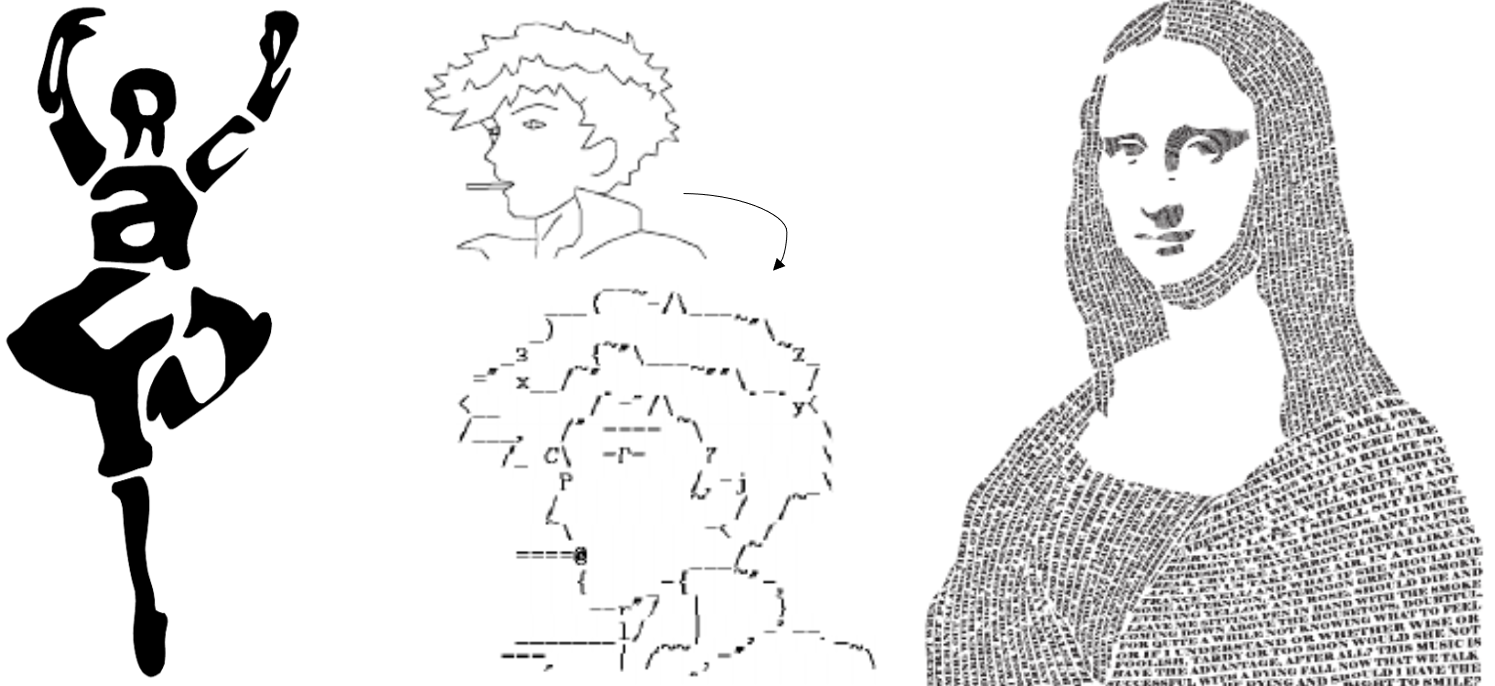
\includegraphics[width=0.8\textwidth]{figures/calligram.png}
	\caption{以字符为基础的文字诗图形排样方法。左:字母变形~\supercite{Zou2016};中:Ascii字符艺术~\supercite{Xu2010};右:文段依向量场排布~\supercite{Moharik2011}。}
	\label{fig:calligram}
\end{figure}

\bigbreak
图形学的相关工作尽管与本文所要探索的内容在最终效果有一定相似之处,但其主要考虑的是在给定图像上的填充,对艺术性及趣味性的要求往往高于文本可读性,有时会根据区域形状对字体样式进行变形,字的大小与位置通常仅与填充的需求相关~\supercite{Kyprianidis13}。而多分辨率词云所依赖的数据为具有双层结构的词集,最终布局是灵活的,且其对于文字的可识别性有更高的要求,需要通过字的大小反映词频等重要性指标,以此辅助完成文本分析任务。在处理上下层词云的布局关系时,我们在一定程度上借鉴了图像拼接的基本思路,例如先分割再排布、对区域进行预处理等等。而对于词云这一特殊可视化的布局,我们进行了更为深入的考量。


\subsection{媒介相关方法}
对于一些具有特殊物理特性的显示媒介来说,人们在不同视角下能够观察到的仅为其整体显示中的局部。在此基础上,人们就可以在同一个媒介中隐藏不同层次的信息。例如,装饰画中常见的光栅立体图~\supercite{Yitzhak2018}就利用了塑料光栅板对光线的折射与衍射,改变图像上各点光线传播的方向,使人的双眼分别观察不同的图片,在视位差的作用产生立体感。类似地,Kim等人注意到了扭曲向列型液晶显示屏(TN-LCD)在不同观察角度下对应的颜色亮度不一致。利用这种感知差异,他们通过将两幅图像同时在时间频域与空间频域逐像素交错显示的方法,制造出一系列从不同方位看有不同内容的图片~\supercite{Kim2012}。媒介相关的多分辨率技术巧妙地借助了显示硬件的物理特性,但受限于此,不利于推广。此外,他们多依赖于观察者视角的切换,因此难以建立起明确的交互语义。相对而言,上文所述的图形排布与嵌套以及频域滤波的方法则是通过观察者与观察对象的距离而改变产生不同的视图,人们在由远及近时具有先概览、后细节的自然交互,因此更适合于可视化。

\bigbreak
需要仔细区分的是,我们所研究的多分辨率技术与缩放有所区别。缩放能改变显示的信息层级,模拟观察距离或语义层次的改变,让用户能够从概览中找出感兴趣的区域再进一步定位~\supercite{Cockburn2009}。但它动态地改变了用户的视图,不利于多人合作的场景,因而不做探讨。在时间序列可视化中,也有“多分辨率”的说法。这指的是在一个视图整体中同时展示不同时间粒度下的聚合信息~\supercite{Hao2007},亦不属本文所研究范畴。

\section{词云}
词云在引言中已有介绍,以下回顾词云的代表性布局算法以及其在文本可视分析中的应用案例。

\subsection{布局算法}
词云的布局算法一直是研究的热点。Viegas等人~\supercite{Viegas2009}最早提出Wordle的概念,突破了传统词云无法旋转、样式单一等局限,具有很强的艺术性。他们在布局时使用的是贪心算法:首先为每一个词语随机设定初始位置,或按照字母序沿横轴均匀排布,或围绕中心发散排布;每当词与词的边界框产生交叠,便沿螺旋线方向相应调整词语位置。而Rolled-out Wordle~\supercite{Strobelt2012}改进了Wordle迭代更新时逐元素检查是否交叠的策略,换以图像逐行扫描或沿圆心放射扫描,以此保证整体布局的紧凑性。不少布局算法还考虑了语义,使关联强的词语聚簇在一起。Cui等人~\supercite{Cui2010}提出了自适应的力导向词云布局算法,先为各大意群随机设定位置,以此为中心初始化词语,再通过引力与斥力的模拟微调布局。Wu等人~\supercite{Wu2011}则是以MDS投影设定各词语初始位置,维护基于语义关联的距离度量,再通过线裁剪去除空白部分。特别地,一部分工作在自动化布局的基础上为设计者提供交互修改的自由度,如支持鼠标选择移动的ManiWordle\supercite{Koh2010}和支持手写笔的WordlePlus~\supercite{Jo2015},以及进一步维护紧凑布局的EdWordle~\supercite{Wang2018}等。

形变词云(Morphable Word Cloud)类似于文字诗,支持用户指定词云外层的轮廓形状,能够产生多分辨率的效果。Chi等人~\supercite{Chi2015}将每个词视为有质量的刚体,通过动力学原理为布局添加边界等限制进行迭代。借助物理模型,他们不仅有效限制了词云的形状,还为展示词云随时间的变化提供了流畅的过渡。ShapeWordle~\supercite{Wang2020}延拓了以往空隙填充算法中使用的螺旋线,通过外层轮廓对应的向量场为词云所在区域重新定义了距离场,使得在迭代过程中词语能以接近外层轮廓的螺旋线调整。

对词云布局的评价标准是多样化的。参考Barth等人~\supercite{Barth2014}的工作,评估一个词云布局算法的优劣可从以下几个角度考虑:(1)布局紧凑性,即是否充分使用空白的区域;(2)布局均匀性,即词云的位置是否足够随机,留下均匀分布的空白区域;(3)维护语义的能力,相似语境下的的词语能否聚到一起。我们无意研究一个新的词云生成算法,而是考虑在现有算法的基础上加入多分辨率技术,使用户可以在不同场景下选择更为合适的基础词云形式。本文在具体实现时主要利用了基于贪心策略的算法,而对细节部分的布局则考虑了一些形状上的限制,第~\ref{sec:refinement}节将具体讨论。

\subsection{文本可视分析}
尽管词云是最易于理解的可视化方法之一,但利用词云完成分析型任务还存在诸多挑战。例如,字号并非编码定量型数据的最佳视觉通道~\supercite{Munzner2014}。对于处于同一级别的词语,尽管它们的字号是一样的,但字数更长的词所占的面积会更大,潜在地影响了人的判断,营造出它更为``关键''的假象;而词语的布局位置与词本身没有明确的对应关系,当用户有特定感兴趣词汇时并难以快速定位搜索~\supercite{Lohmann2009};此外,由于脱离了上下文,人们难以从零星的关键词中构建完整的理解~\supercite{Viegas2008}。近期,Felix等人~\supercite{Felix2018}基于不同的分析任务对比了几种展示关键词的设计选择,认为词云更适合于抽象的文本分析任务,如概括与理解话题,而它对于精确的数据分析任务并非是最有效的。

为了应对以上挑战,一方面,许多布局算法将强关联的词语聚合在相邻区域以增强用户对整体概念的把握和理解,而另一方面,一些可视分析工作结合具体的任务需求,将词云与其他可视化形式有机结合,挖掘交互探索的可能性,使词云综合发挥作用。SentenTree~\supercite{Hu2017}借助自然语言处理中的语义解析技术,用树的形式展现社交媒体中的热门话题及其分支,保留了短语逻辑的完整性。Parallel Word Clouds~\supercite{Collins2009}以词垂直布局作为平行坐标轴对比数据的不同层面。本研究所关注的大屏多分辨率词云属于对大规模词云布局的底层可视化技术,适用于时序语料以及大型非结构化文本数据。在这一主题下,涌现了相当多的工作。SparkClouds~\supercite{Lee2010}将词语与迷你折线图合并为基础布局单元;WordStream~\supercite{Dang2019}以主题河流图的形式展现了关键词的变迁。此外,少数工作探索了大型语料库的渐进性探索。TexTonic~\supercite{Paul2019}借用地图的隐喻,为维基百科这样的大规模文本库提供了用户主导的交互式词云可视化,将原始文本、片段聚类、关键词以多层次地图疆界的方式结合(见图~\ref{fig:textonic})。

\begin{figure}[htbp]
	\centering
	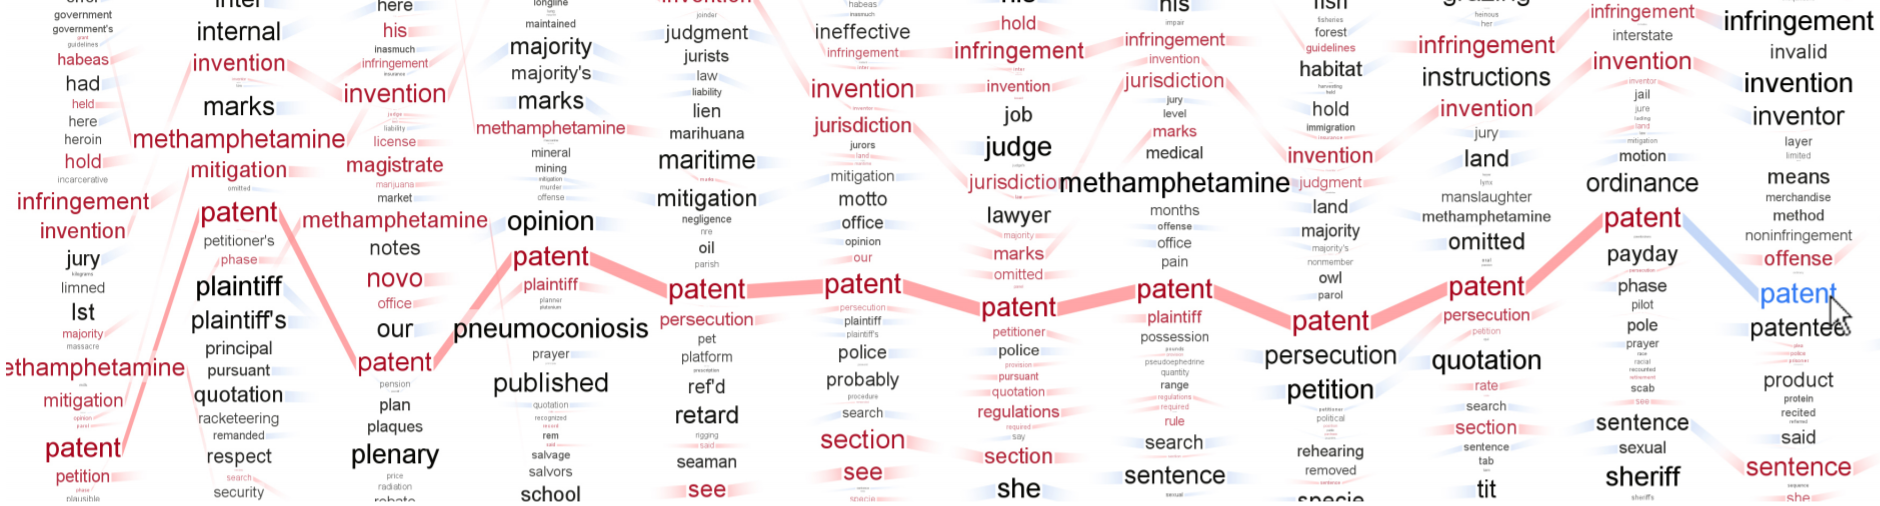
\includegraphics[width=\textwidth]{figures/parallel.png}
	\caption{Parallel Word Clouds~\supercite{Collins2009}:大型时序平行坐标词云。}
	\label{fig:textonic}
\end{figure}

\begin{figure}[htbp]
	\centering
	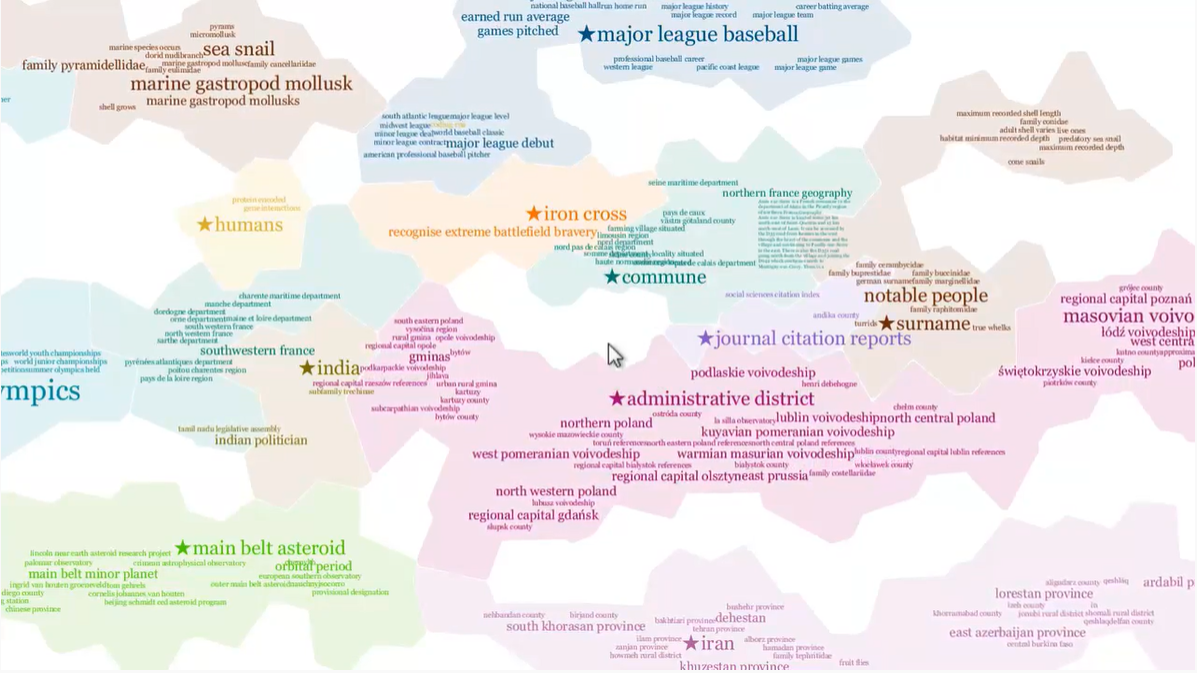
\includegraphics[width=\textwidth]{figures/TexTonic.png}
	\caption{TexTonic~\supercite{Paul2019}:基于地图词云的大型文本交互探索系统。}
	\label{fig:textonic}
\end{figure}
